\chapter{Fondamenti Teorici}
\label{ch:fondamenti}

In questo capitolo verranno trattati alcuni fondamenti teorici necessari per la
comprensione dell'elaborato. Si procederà con un'analisi sullo stato dell'arte della
libreria in oggetto e una breve introduzione al funzionamento delle Reconfigurable
Intelligent Surfaces, per poi passare ad una panoramica generale sulle tecniche
di parallel computing, con particolare attenzione alle differenze tra CPU e GPU e
tra i framework \textit{CUDA} e \textit{OpenCL}. Infine, si presenteranno i presupposti
limiti teorici e risultati attesi.

% do not wrap citation
\section[Modello delle Reconfigurable Intelligent Surfaces]{Modello delle
Reconfigurable Intelligent Surfaces\cite{cooperis}}
\label{sec:statodellarte}

\begin{figure}[!htbp]
  \begin{minipage}[t]{0.5\linewidth}
    \centering
    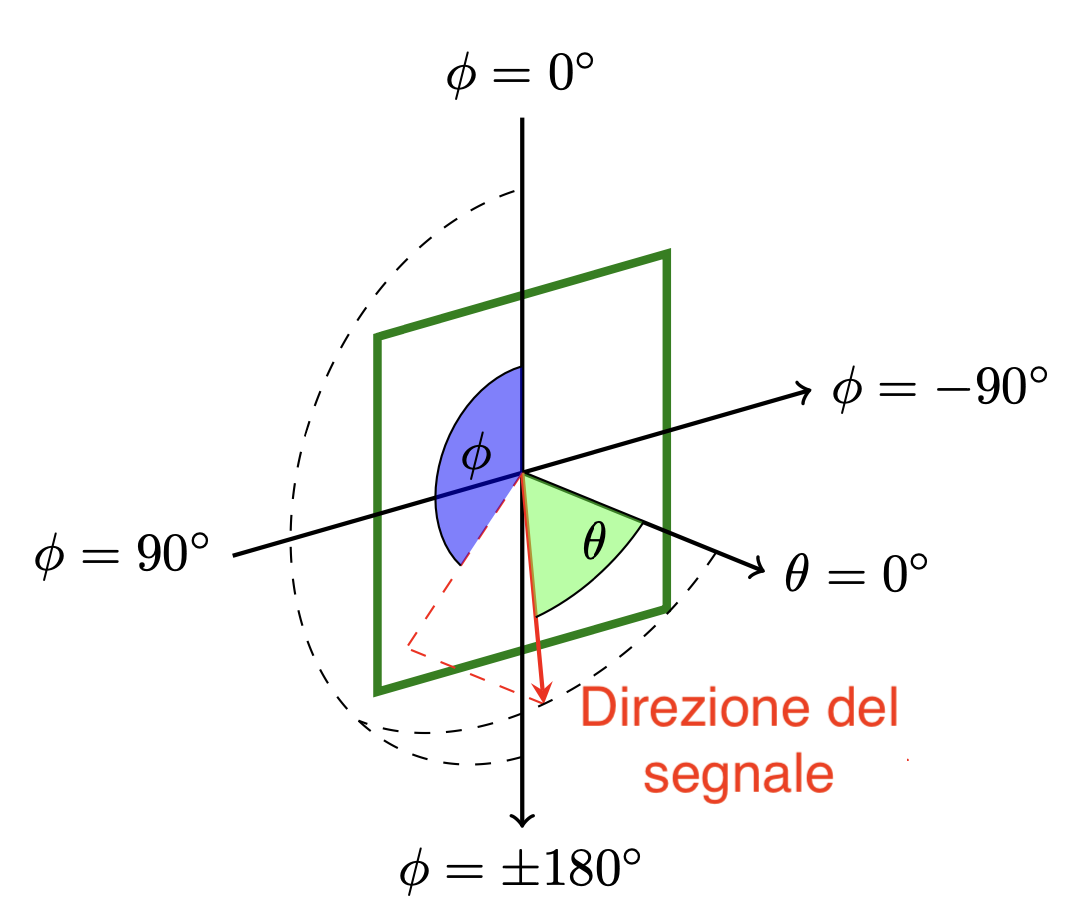
\includegraphics[width=8cm]{images/examples/coords.png}
    \begin{adjustwidth}
      {0pt}{5pt}
      \begin{varwidth}
        {8cm}
        \caption{Angoli di incidenza e riflessione del segnale rispetto la RIS\cite{cooperis}}
        \label{fig:coords}
      \end{varwidth}
    \end{adjustwidth}
  \end{minipage}
  \begin{minipage}[t]{0.5\linewidth}
    \centering
    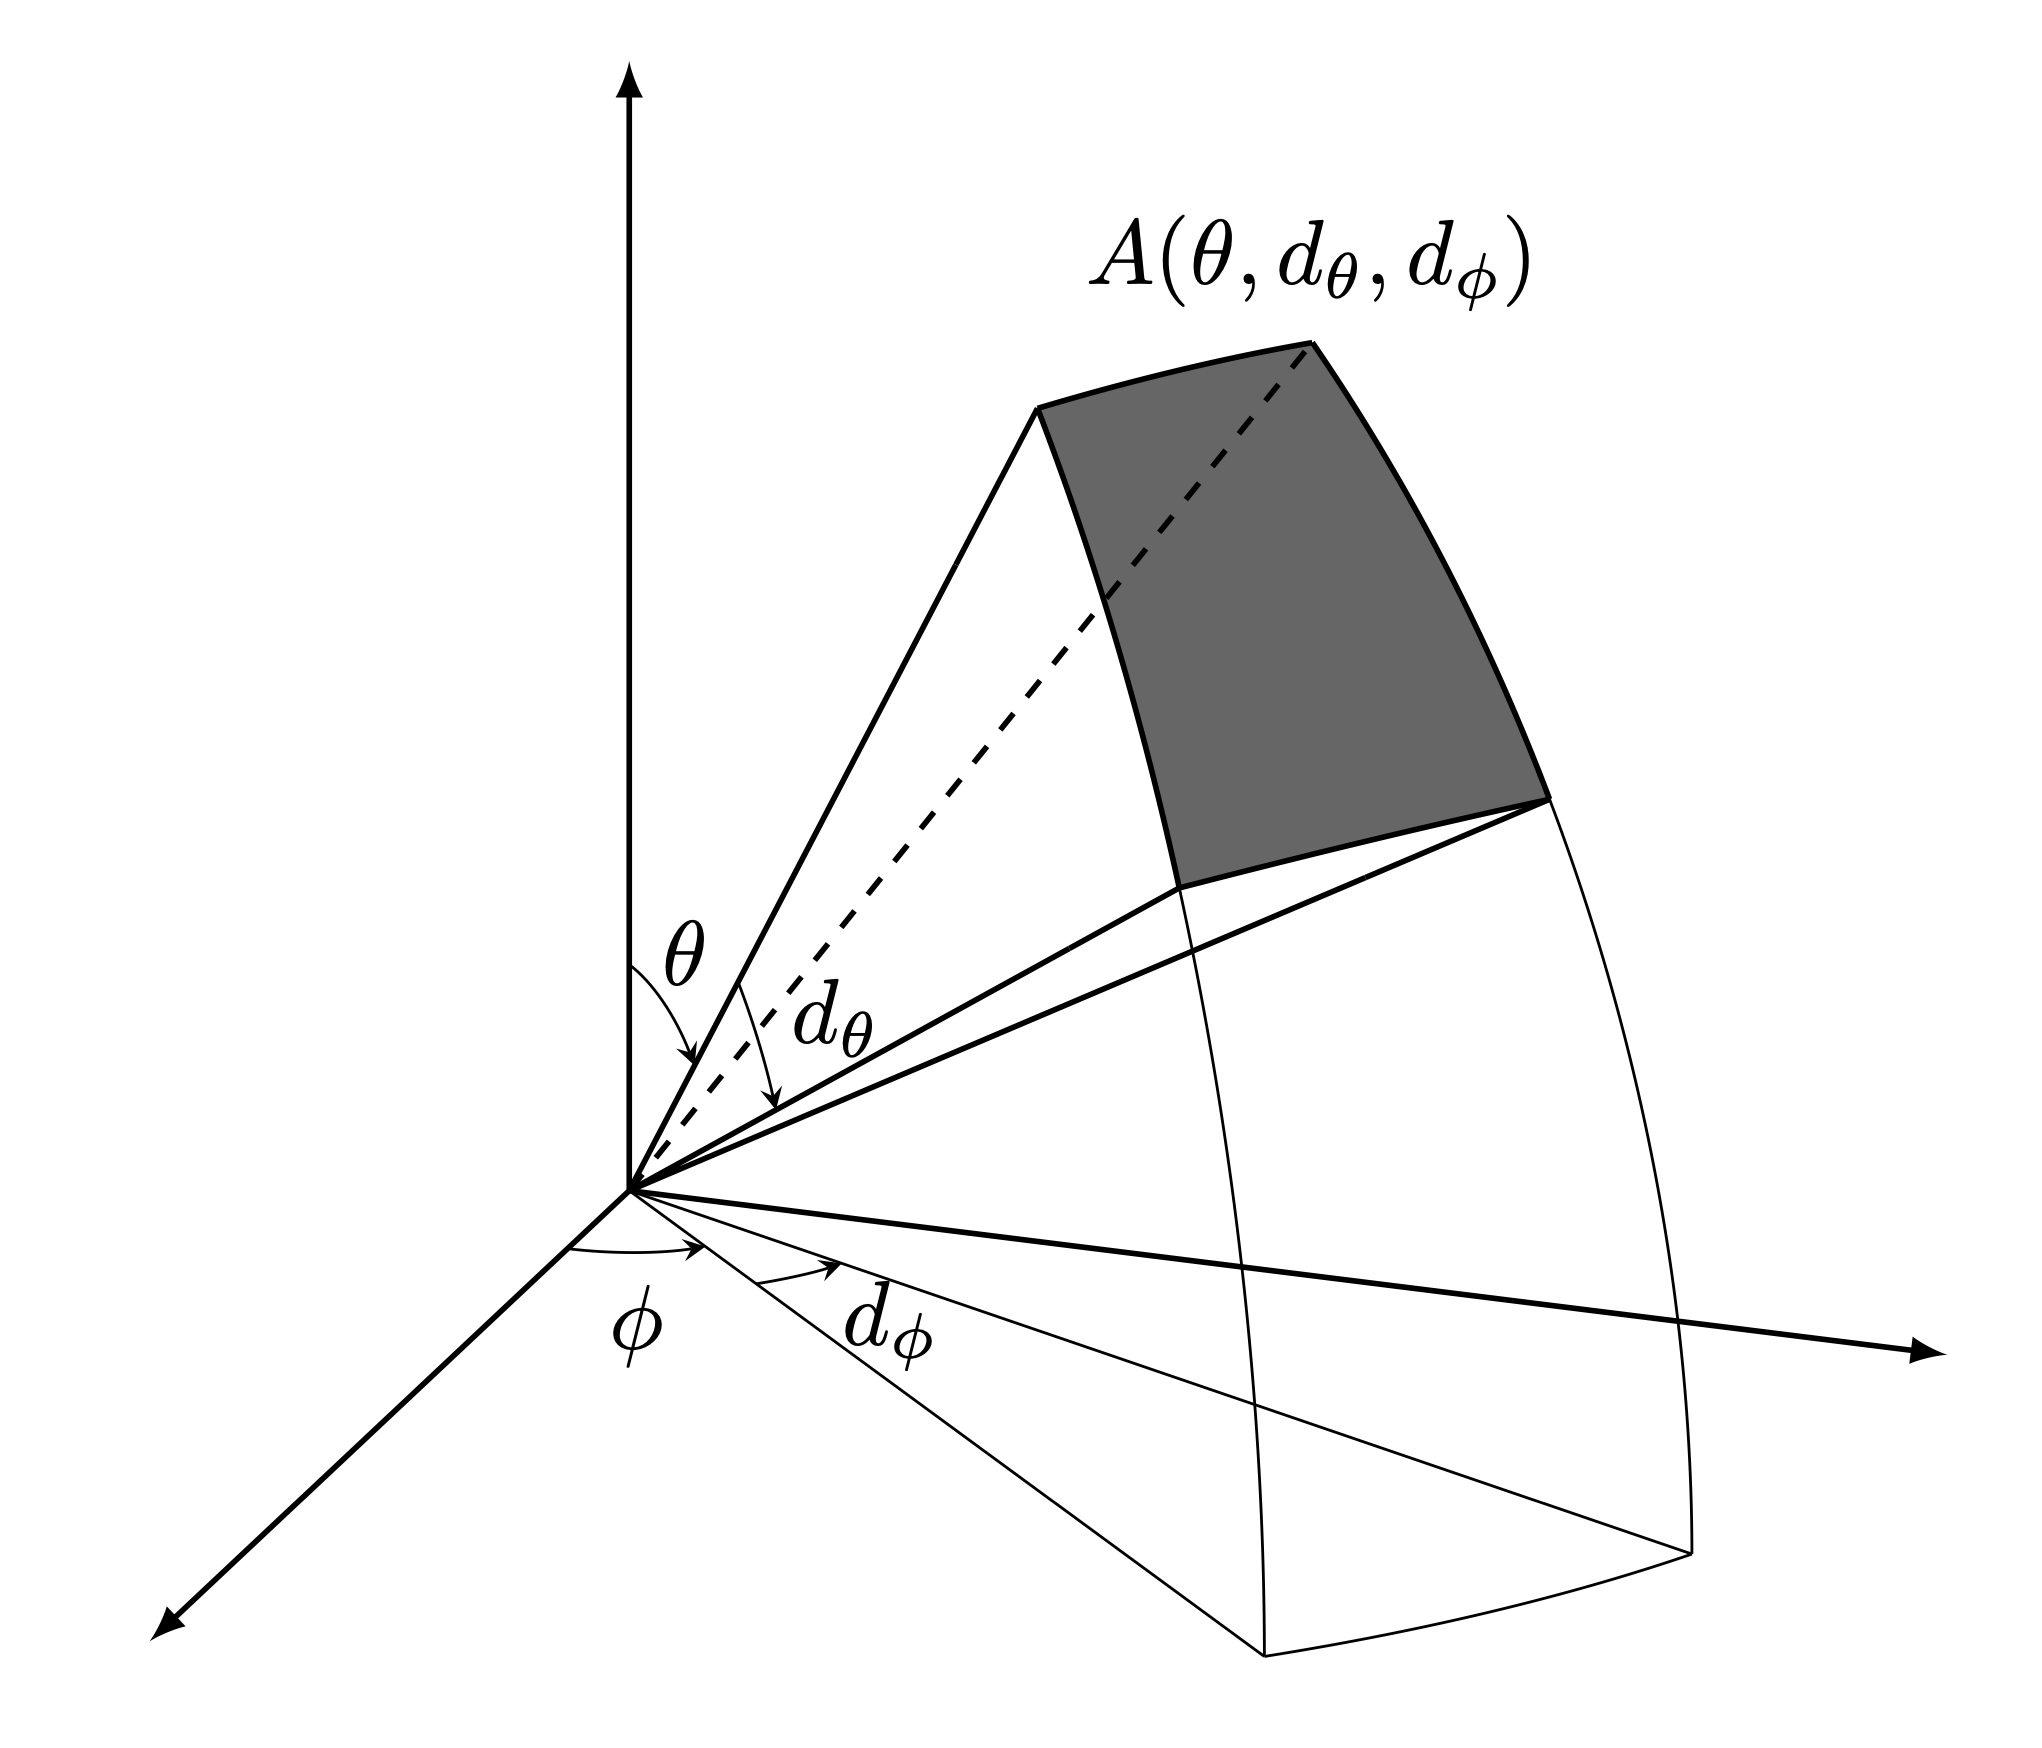
\includegraphics[width=8cm]{images/examples/spherical-element.png}
    \begin{adjustwidth}
      {5pt}{0pt}
      \begin{varwidth}
        {8cm}
        \caption{Esempio grafico di un elemento sferico e la sua
        discretizzazione\cite{cooperis}}
        \label{fig:spherical-elem}
      \end{varwidth}
    \end{adjustwidth}
  \end{minipage}
\end{figure}

L'apprendimento delle Reconfigurable Intelligent Surfaces è fondamentale per comprendere
al meglio quali sono le potenziali criticità e gli eventuali punti di ottimizzazione
della libreria \textit{CoopeRIS}, e di conseguenza di questo elaborato. Come già
accennato nel capitolo \ref{subsec:risframework}, le Reconfigurable Intelligent Surfaces
sono dispositivi che permettono di modificare la riflessione di un segnale appartenente
ad un canale di comunicazione tra un trasmettitore e un ricevitore, al fine di
migliorare la qualità del segnale ricevuto. Questi dispositivi sono composti da un
insieme di elementi radianti, che possono essere attivati per modificare la
riflessione del segnale in arrivo. La somma dei contributi di riflessione di ogni
singolo elemento radiante permette di ottenere un segnale riflesso nitido e direzionato
verso il ricevitore, migliorando così la qualità del segnale ricevuto. La libreria
\textit{CoopeRIS} supporta esclusivamente le RIS passive, ovvero quelle che non permettono
di amplificare il segnale, ma che ne migliorano solo la riflessione. Nel contesto
di una simulazione il parametro più rilevante è $\textbf{G}$, il guadagno
isotropico della RIS dettato dall'equazione \ref{eq:gain}, il quale permette di valutare
la qualità del segnale ricevuto e pertanto la qualità della comunicazione tra trasmettitore
e ricevitore. Esso non è altro che la somma della potenza in \ref{eq:power} del
segnale riflesso in ogni direzione del ricevitore $rx$, normalizzata rispetto all'area
$A(\vartheta, d_{\theta}, d_{\phi})$ del corrispettivo elemento sferico,
definito nell'equazione \ref{eq:area-spherical-element}. Si noti che, per
necessità di calcolo, l'area degli elementi sferici, e di conseguenza anche
$\Theta_{m,n}$ e $\Phi_{m,n}$, deve essere obbligatoriamente resa discreta e la loro
risoluzione angolare è posta pari a $d_{\theta}$ e $d_{\phi}$, rappresentata in
figura \ref{fig:spherical-elem}. In equazione \ref{eq:phase-phi} è definito $\Phi
_{m,n}$ per elemento radiante in posizione $m$, $n$ dato l'angolo di incidenza
$\phi_{i}$ e riflessione $\phi_{r}$. Esso rappresenta lo sfasamento del segnale dovuto
alla attuale configurazione della RIS. In equazione \ref{eq:phase-theta} è
invece denotato lo sfasamento $\Theta_{m,n}$, il quale descrive lo sfasamento dovuto
alla posizione del trasmettitore e ricevitore. Questa differenziazione consente
il calcolo del guadagno della RIS nella condizione in cui l'attuale
configurazione della RIS sia stata determinata con angoli di incidenza e
riflessione dissimili rispetto le attuali posizione del trasmettitore e
ricevitore. Questa combinazione di fattori è il motivo per cui i contributi dei due
sfasamenti sono sommati nel calcolo del guadagno in equazione \ref{eq:power}.
Infine, in tabella \ref{tab:symbols} sono riportati i simboli e le definizioni utilizzate
per la descrizione delle equazioni sopracitate.

\vspace{1em}

\begin{table}[!ht]
  \centering
  \begin{tabular}{p{.15\textwidth}p{.80\textwidth}}
    \hline
    \textbf{Simbolo}                     & \textbf{Significato}                                                                                                                                                                \\
    \hline
    $M$, $N$                             & Grandezza della matrice di elementi radianti                                                                                                                                        \\
    $m$, $n$                             & Indici di posizione degli elementi radianti                                                                                                                                         \\
    $a_{m,n}$                            & Guadagno di ampiezza del singolo elemento ris (in posizione $m$, $n$, in questo modello si assume sempre pari a $1$)                                                                \\
    $\lambda$                            & Lunghezza d'onda del segnale                                                                                                                                                        \\
    $d_{u}$                              & Distanza tra gli elementi radianti                                                                                                                                                  \\
    $\phi$, $\theta$                     & Azimuth ed elevazione del segnale. Diversi pedici indicano rispettivamente il trasmettitore ($tx$), il ricevitore ($rx$), incidenza ($i$) e riflessione ($r$)                       \\
    $\Phi_{m,n}$, $\Theta_{m,n}$         & Sfasamento del singolo elemento radiante (in posizione $m$, $n$) dovuto rispettivamente alla configurazione della RIS e del segnale data la posizione di trasmettitore e ricevitore \\
    $f(\phi, \theta)$                    & Pattern di scattering dell'elemento radiante (in questo modello si assume sempre pari a $1$)                                                                                        \\
    $\textbf{P}_{\phi_{rx},\theta_{rx}}$ & Potenza del segnale riflesso in uscita                                                                                                                                              \\
    $\textbf{G}$                         & Guadagno normalizzato della RIS                                                                                                                                                     \\
    $A(\theta, d_{\theta}, d_{\phi})$    & Area di un elemento sferico per un elevazione $\theta$ e per una risoluzione angolare di elevazione e azimuth $d_{\theta}$ e $d_{\phi}$                                             \\
    \hline
  \end{tabular}
  \caption{Tabella dei simboli}
  \label{tab:symbols}
\end{table}

\begin{equation}
  \label{eq:phase-phi}\Phi_{m,n}= \frac{2\pi d_{u}}{\lambda}[n(\cos{\phi_{r}\sin{\theta_{r}}}
  -\cos{\phi_{i}}\sin{\theta_{i}})+m(\sin{\phi_{r}}\cos{\theta_{r}}-\sin{\phi_{i}}
  \cos{\theta_{i}})]
\end{equation}

\begin{equation}
  \label{eq:phase-theta}\Theta_{m,n}= \frac{2\pi d_{u}}{\lambda}[n(-\cos{\phi_{rx}\sin{\theta_{rx}}}
  +\cos{\phi_{tx}}\sin{\theta_{tx}})+m(-\sin{\phi_{rx}}\cos{\theta_{rx}}+\sin{\phi_{tx}}
  \cos{\theta_{tx}})]
\end{equation}

\begin{equation}
  \label{eq:power}\textbf{P}_{\phi_{rx},\theta_{rx}}= \left|\sum_{m=0}^{M-1}{\sum_{n=0}^{N-1}{f(\phi_{tx}, \theta_{tx})f(\phi_{rx},\theta_{rx})a_{m,n}e^{-j(\Phi_{m,n}+\Theta_{m,n})}}}
  \right|^{2}, \forall \phi_{rx}, \theta_{rx}
\end{equation}

\begin{equation}
  \label{eq:area-spherical-element}A(\theta, d_{\theta}, d_{\phi})=
  \begin{cases}
    d_{\phi}(1-\cos{\frac{d_{\theta}}{2}})                                         & \text{se }\theta = 0                 \\
    d_{\phi}(\cos{\theta-\frac{d_{\theta}}{2}}- \cos{\theta+\frac{d_{\theta}}{2}}) & \text{se }0 < \theta < \frac{\pi}{2} \\
    d_{\phi}(\theta-\frac{d_{\theta}}{2})                                          & \text{se }\theta = \frac{\pi}{2}     \\
  \end{cases}
\end{equation}

\begin{equation}
  \label{eq:gain}\textbf{G}=\textbf{P}\frac{2\pi}{(\textbf{P}^{\top}\cdot
  \mathds{1})^{\top}\cdot A(\vartheta, d_{\theta}, d_{\phi})}
\end{equation}

\section{Parallel Computing}
\label{sec:parallelcomputing}

Con il termine \textit{parallel computing} si intende la divisione di un
problema in sotto-problemi che possono essere risolti in parallelo su più unità
di calcolo. Un unità di calcolo può essere un core di una CPU, un core di una
GPU, un thread di un processore o un processore dedicato. Questa divisione
permette ai calcolatori dotati di più unità di calcolo di risolvere problemi di
dimensioni maggiori in tempi molto più brevi rispetto a calcolatori che non
implementano il parallelismo. La loro comparsa è stato un traguardo storico e fondamentale
per lo sviluppo delle moderne tecnologie informatiche. Questo capitolo si
propone di fornire una panoramica generale sulle tecniche di parallel computing,
con particolare attenzione alle differenze tra CPU e GPU e tra i framework \textit{CUDA}
e \textit{OpenCL}.

\subsection{CPU vs. GPU}
\label{subsec:cpuvsgpu}

Le CPU e le GPU sono due tipologie di unità di calcolo che distinguono per
architettura, scopo e prestazioni. La loro differenziazione nasce dalla natura
delle operazioni che possono essere eseguite su di esse. Generalmente le CPU sono
progettate per eseguire operazioni complesse e molto variegate, forniscono un'architettura
di calcolo più generica e flessibile (\textit{general purpose}) e per questo possono
eseguire parallelamente un numero limitato di operazioni. Le GPU, d'altra parte,
sono specializzate nel parallelizzare le operazioni su grandi quantità di dati, al
costo di una minore flessibilità. Per questa ragione, se prese singolarmente, le
performance delle unità di calcolo sono inferiori rispetto a quelle delle CPU. Per
poter meglio evidenziare le differenze tra le due piattaforme, è necessario
introdurre i concetti di SISD, SIMD e SIMT.

\paragraph{Single Instruction, Single Data (SISD)}
\label{para:simd}

Il modello SISD è quello del calcolo tradizionale ed è il più elementare tra i tre.
Consiste in un'architettura sequenziale in cui un singolo processore esegue un'istruzione
per volta su un singolo dato. Questo modello è tipico delle CPU, che possono
però gestire più thread in parallelo grazie alla presenza di più core
indipendenti che eseguono diverse istruzioni su diversi dati. Questa tecnica è detta
\textit{multi-threading} e permette di eseguire più processi in parallelo. Data la
sua semplicità, il modello SISD permette di ottenere performance elevate su
problemi che richiedono un'elaborazione sequenziale di dati, come ad esempio i sistemi
operativi o i programmi di uso generale.

\begin{figure}[h!]
  \centering
  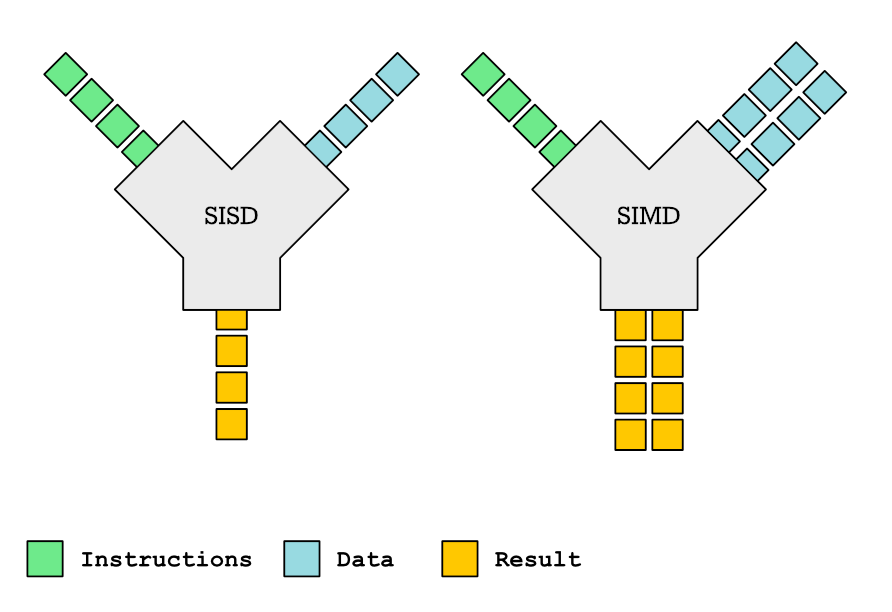
\includegraphics[width=.40\linewidth]{images/examples/sisd-simd.png}
  \caption{Differenza tra SISD e SIMD}
  \label{fig:sisd-simt} \footnotesize{Fonte: \url{https://johnnysswlab.com/crash-course-introduction-to-parallelism-simd-parallelism/}}
\end{figure}

\paragraph{Single Instruction, Multiple Data (SIMD)}
\label{para:simd}

Come suggerisce il nome, la tecnica SIMD permette di eseguire un'istruzione per elaborare
più dati simultaneamente. Questa tecnica è particolarmente efficace per eseguire
operazioni identiche su grandi quantità di dati, come calcoli vettoriali, o
generalmente nelle strutture linearizzabili, come le matrici. La sua
implementazione trova spazio sia nelle GPU che nelle CPU, attraverso l'uso di apposite
istruzioni definite dall'ISA (Instruction Set Architecture) del processore.

\paragraph{Single Instruction, Multiple Threads (SIMT)\cite{generalpurposegpu}}
\label{para:simt}

La tecnica SIMT è una variante della tecnica SIMD che estende il concetto di parallelismo
a livello di thread. Il suo funzionamento consiste in più thread, raggruppati in
gruppi detti \textit{warps}. Ogni thread possiede il proprio insieme di registri
e il proprio contesto, ma condividono l'istruzione da eseguire all'interno del
warp. In questo modo, tutti i thread del \textit{warp} eseguono la medesima istruzione,
ma con dati diversi. Se, per l'architettura del nostro programma, non tutti i thread
all'interno del \textit{warp} soddisfano un controllo di flusso, ad esempio in un
branch condizionale, allora i thread che non rispettano la condizione vengono
disattivati, mentre quelli che soddisfano la condizione continuano l'esecuzione.
Questo comportamento è detto \textit{divergenza} e può portare a un rallentamento
delle prestazioni del programma, in quanto i thread disattivati devono comunque
attendere il completamento dell'istruzione da parte dei thread attivi, che a loro
volta devono attendere il completamento delle istruzioni presenti nell'altro ramo
del branch condizionale. Le GPU sono i dispositivi che implementano questa
tecnica che è alla base del loro funzionamento.

\vspace{1em}

Queste tecniche sono alla base del funzionamento delle CPU e delle GPU, e
evidenziano quali sono le aree di applicazione di ciascuna di esse. Di seguito,
a titolo esemplificativo, viene riportato un esempio implementativo di due funzioni
di somma di vettori in pseudo-codice, una per CPU (\ref{alg:sumvectorscpu}) e
una per GPU (\ref{alg:sumvectorsgpu}).

\begin{figure}[h!]
  \vspace{1em}
  \begin{algorithm}
    [H]
    \caption{Somma di vettori tramite CPU}
    \label{alg:sumvectorscpu}
    \begin{algorithmic}
      \Function{sum\_vectors\_cpu}{A, B, C} \For{$i \gets 0$ to $n$} \State
      $C[i] \gets A[i] + B[i]$ \EndFor \EndFunction
    \end{algorithmic}
  \end{algorithm}
  \vspace{1em}
\end{figure}

Possiamo notare come la funzione \texttt{sum\_vectors\_cpu} esegua la somma di
due vettori $A$ e $B$ e memorizzi il risultato in un terzo vettore $C$ tramite
un ciclo \texttt{for} che scorre tutti gli elementi dei vettori. Questo
approccio è sequenziale ed è quello classico adotto per l'esecuzione su CPU.

\begin{figure}[h!]
  \vspace{1em}
  \begin{algorithm}
    [H]
    \caption{Somma di vettori tramite GPU}
    \label{alg:sumvectorsgpu}
    \begin{algorithmic}
      \Function{sum\_vectors\_gpu}{A, B, C} \State $i \gets \textit{threadId}$ \State
      $C[i] \gets A[i] + B[i]$ \EndFunction
    \end{algorithmic}
  \end{algorithm}
  \vspace{1em}
\end{figure}

La funzione \textit{sum\_vectors\_gpu}, invece, esegue lo stesso compito tramite
sole due istruzioni, senza necessità di un ciclo \texttt{for}. Questo è possibile
proprio per l'architettura SIMT, poiché $n$ istanze della funzione \texttt{sum\_vectors\_gpu}
vengono eseguite, con $n$ pari al numero di elementi da sommare. Ogni istanza, o
thread, ha associato un indice $i$ che identifica l'elemento del vettore su cui deve
operare, che si ottiene tramite il contesto del thread stesso. In gergo, questa
funzione viene definita \textit{kernel}, ovvero una funzione compilata nel
codice macchina specifico per la GPU, la quale sarà poi invocata dal codice \textit{host},
ovvero il programma che esegue sulla CPU e che gestisce l'esecuzione sul \textit{device}
GPU, tramite le API predisposte dal framework di riferimento.

\subsection[\textit{CUDA} vs. \textit{OpenCL}]{\textit{CUDA} vs. \textit{OpenCL}\cite{cuda}\cite{opencl}\cite{cudavsopencl}}
\label{subsec:cudavsopencl}

\textit{CUDA} e \textit{OpenCL} sono due framework per il parallel computing
piuttosto diffusi e utilizzati per sfruttare le potenzialità delle GPU. Entrambi
i framework permettono di scrivere codice in \textit{C/C++} per creare procedure
eseguibili su GPU, ma differiscono per finalità e prestazioni. \textit{CUDA} è noto
per essere più facile da utilizzare e offre un livello di ottimizzazione superiore.
Tuttavia, questo vantaggio comporta un compromesso significativo: la
compatibilità è limitata esclusivamente alle GPU prodotte da NVIDIA. Questa restrizione
deriva dal fatto che \textit{CUDA} è stato sviluppato e mantenuto interamente da
NVIDIA, rendendolo utilizzabile solo con le loro GPU. \textit{OpenCL}, invece, è
un framework più generico e flessibile, che permette di programmare virtualmente
su tutte le piattaforme GPU, ma al costo di un \textit{overhead} maggiore
rispetto a \textit{CUDA} poiché, ad esempio, è necessario compilare le funzioni \textit{kernel}
a runtime, mentre in \textit{CUDA} questo passaggio è già gestito in fase di
compilazione. Entrambi sono molto diffusi e utilizzati, e la scelta tra uno e l'altro
dipende dalle esigenze del programmatore e dal progetto. Anche se presente, la
loro differenza di prestazioni è trascurabile se si confrontano i risultati in
implementazioni dove le GPU trovano la loro massima efficacia rispetto alle CPU
e se si sanno sfruttare sapientemente le loro potenzialità.

\section{Limiti teorici}
\label{sec:limititeorici}

Sebbene il calcolo parallelo sia una tecnica molto potente, presenta dei limiti
invalicabili che pongono dei vincoli sulle massime prestazioni ottenibili. La comprensione
di questi limiti è fondamentale per la progettazione di sistemi paralleli efficienti,
soprattutto per individuare le parti del codice che sono strategicamente più
importanti da ottimizzare. Il principio di maggiore rilevanza per questo elaborato
è rappresentato dalla Legge di Amdahl, il quale rivestirà un ruolo preponderante
nell'analisi statica condotta sulla libreria in oggetto, come discusso nel paragrafo
\ref{sec:ottimizzazione}. Questo principio sarà fondamentale per identificare le
sezioni del codice che richiedono particolare attenzione e ottimizzazione, consentendo
un miglioramento mirato delle prestazioni complessive del sistema.

\subsection{Legge di Amdahl}
\label{sec:amdahl}

La Legge di Amdahl, formulata da Gene Amdahl nel 1967, è un principio
fondamentale pessimista che descrive un limite superiore al miglioramento
teorico delle prestazioni di un sistema in seguito all'aggiunta di risorse
parallele in funzione della frazione del problema che può beneficiare della
parallelizzazione. La sua formulazione è la seguente:

\begin{equation}
  S(N) = \frac{1}{(1 - P) + \frac{P}{N}}
\end{equation}

Dove:
\begin{itemize}
  \item $S(N)$ è il miglioramento teoretico ottenuto con $N$ processori.

  \item $N$ è il numero di processori.

  \item $P$ è la frazione del problema che può beneficiare della parallelizzazione.
\end{itemize}

In sintesi, questo modello prevede che all'aumentare del numero di processori,
il miglioramento ottenuto con l'aggiunta di un processore aggiuntivo tende a
zero. Per questa ragione, nel paradigma della parallelizzazione, è più conveniente
parallelizzare le parti del codice che richiedono più tempo di esecuzione che aggiungere
processori per parallelizzare parti del codice che richiedono poco tempo di esecuzione.
Inoltre, non sono considerati altri fattori che possono influenzare le prestazioni
di un sistema parallelo, come ad esempio la latenza di comunicazione tra i
processori o il tempo tecnico necessario per l'avvio, la sincronizzazione e la terminazione
dei processi paralleli.